\documentclass[12pt, a4 paper]{article}
% Set target color model to RGB
\usepackage[inner=2.0cm,outer=2.0cm,top=2.5cm,bottom=2.5cm]{geometry}
\usepackage{setspace}
\usepackage[rgb]{xcolor}
\usepackage{environ}
\usepackage{verbatim}
\usepackage{subcaption}
\usepackage{outlines}
\usepackage{enumitem}
\usepackage{amsgen,amsmath,amstext,amsbsy,amsopn,tikz,amssymb,tkz-linknodes}
\usepackage{fancyhdr}
\usepackage{pgfplots}
\usepackage{mathtools}
\usepackage[colorlinks=true, urlcolor=blue,  linkcolor=blue, citecolor=blue]{hyperref}
\usepackage[colorinlistoftodos]{todonotes}
\usepackage{rotating}

\linespread{1.6} % Double Line Spacing
\usetikzlibrary{arrows.meta,intersections,calc}

\hypersetup{%
pdfauthor={Vignesh Ravibaskar},%
pdfcreator={PDFLaTeX},%
pdfproducer={PDFLaTeX},%
}

% Our custom enumerate labelling, just making the outlines bold basically
\setlist[enumerate,1]{label=\textbf{\arabic*}}
\setlist[enumerate,2]{label=\textbf{({\alph*})}}
\setlist[enumerate,3]{label=\textbf{({\roman*})}}

\title{Complex Numbers}
\author{Derek, Vignesh}
\date{2020}

\newcommand{\comm}[1]{}
\NewEnviron{answer}{\vspace{3mm} \\ \color{blue} {\BODY} \color{black}}
% \NewEnviron{answer}{\color{blue} \comm{\BODY} \color{black}} % Use this method to hide all answers

\begin{document}

\maketitle

\textbf{COMPLEX NUMBERS [90 Marks]}
\begin{outline}[enumerate]
	\1 Solve the following: %Question 1

	\2 Given that $z=a+ib$ and $w=c+id$, where $a,b,c,d \in \mathbb{R}$, %Question 1a

	\3 Show that $(zw)^*=z^*w^*$. \hfill[2]
	\begin{answer}
		We will perform algebraic manipulation of the given complex numbers using $a,b,c,d$
		\begin{align*}
			(zw)^* & = [(a+ib)(c+id)]^* = [ac-bd+(bc+ad)i]^* = ac-bd-(bc+ad)i \\
			z^*w^* & = (a-ib)(c-id) = ac-bd-(bc+ad)i\quad\textrm{(Shown)}
		\end{align*}
	\end{answer}
	\3 Hence, show that $(vzw)^*=v^*z^*w^*$ where $v \in \mathbb{C}$.\hfill[1]
	\begin{answer}
		Using the identity from above:
		\begin{align*}
			(vzw)^*            & = v^*(zw)^*                      \\
			\therefore (vzw)^* & = v^*z^*w^*\quad\textrm{(Shown)}
		\end{align*}
		OR Let $v=x+iy$ where $x,y \in \mathbb{R}$
		\begin{align*}
			(vzw)^*   & = [(x+iy)(ac-bd+(bc+ad)i)]^*                      \\
			          & = [acx-bdx-(bc+ad)y+(bc+ad)xi]^*                  \\
			          & = acx-bdx-(bc+ad)y-(bc+ad)xi                      \\
			v^*z^*w^* & = (x-iy)[ac-bd-(bc+ad)i]                          \\
			          & = acx-bdx-(bc+ad)y-(bc+ad)xi\quad\textrm{(Shown)}
		\end{align*}
	\end{answer}

	\2 The locus of a parabola is given by $z=at^2+i(2at)$ for $a,t \in \mathbb{R}$.\\ Show that $|z-a|=|\textrm{Re}(z)+a|$.\hfill[3] %Question 1b
	\begin{answer}
		We will just perform basic algebraic manipulation to prove this. Recall that the magnitude of a positive real number is the number itself and the magnitude of a complex number can be thought of as the distance from the origin of the complex number and is given by the equation $|z|=\sqrt{[\textrm{Re}(z)]^2+[\textrm{Im}(z)]^2}$
		\begin{align*}
			  & |z-a| = |at^2-a+i(2at)| = \sqrt{(at^2-a)^2+(2at)^2} = \sqrt{a^2t^4+a^2+2(at)^2} = at^2 + a \\
			  & |\textrm{Re}(z)+a| = at^2+a \quad\textrm{(Shown)}
		\end{align*}
	\end{answer}

	\2 It is given that $\textrm{Im}(\dfrac{a+bi}{a-bi})=0$ for some $a,b \in \mathbb{R}$. \\ Find the possible values of $\dfrac{a+bi}{a-bi}$.\hfill[3] %Question 1c
	\begin{answer}
		When $\textrm{Im}(\dfrac{a+bi}{a-bi})=0$, it means that the coefficient of $i$ after performing algebraic manipulation of $\dfrac{a+bi}{a-bi}$ is 0. We first multiply the top and bottom of the given fraction with the conjugate of the denominator.
		\begin{align*}
			\frac{a+bi}{a-bi}            & = \frac{(a+bi)(a+bi)}{(a-bi)(a+bi)} = \frac{a^2-b^2+2abi}{a^2+b^2} \\
			\implies 2ab                 & = 0 \implies a=0 \quad\textrm{OR}\quad b=0                         \\
			\therefore \frac{a+bi}{a-bi} & = \pm1
		\end{align*}
	\end{answer}

	\2 For some $a,b \in \mathbb{R}$, $z^2+az-b=0$ has no real roots and $aw^2+bw+a=0$ has two real distinct roots. Given that $a>1$, find an inequality satisfied by $b$. \hfill[3] %Question 1d
	\begin{answer}
		Recall that for any quadratic equation with real coefficients, the discriminant's value,$\Delta$, defines the nature of its roots. Further recall that $\Delta = b^2-4ac$
		\begin{align*}
			\Delta(z^2+az-b)    & = a^2-4(1)(-b) = a^2+4b < 0 \quad\textrm{(no real roots)}         \\
			\Delta(aw^2+bw+a=0) & = b^2-4(a)(a) = b^2-4a^2 >0 \quad\textrm{(2 distinct real roots)}
		\end{align*}
		From the above equations we can glean that $b<\dfrac{-a^2}{4}$ and $b^2>4a^2$ which implies that $b<-2a$ since $a>1\implies a^2>1$. Equating $\dfrac{a^2}{4}=2a$:
		\begin{align*}
			\frac{a^2}{4} & =2a \\
			a(a-8)        & = 0
		\end{align*}
		For $1<a\leq8$, $2a\geq\dfrac{a^2}{4}$ and for $a>8$, $2a\leq\dfrac{a^2}{4}$. This gives us the inequality below:
		\begin{align*}
			\begin{rcases}
			b<-2a, 1<a\leq8       \\
			b<\frac{-a^2}{4}, a>8
			\end{rcases}
		\end{align*}
	\end{answer}

	\2 It is given that $k=\dfrac{a-z^*}{z}+\dfrac{a-z}{z^*}$, where $z=a+ib$ for some $a,b \in \mathbb{R}$.\\Show that $k=\dfrac{2b^2}{a^2+b^2}$.\hfill[3] %Question 1e
	\begin{answer}
		We will just use the equation $z=a+ib$ to solve this equation after making the denominator of the fractions to be $zz^*=|z|^2$
		\begin{align*}
			k = \frac{a-z^*}{z}+\frac{a-z}{z^*} & = \frac{(a-z^*)z^*}{zz^*} +\frac{(a-z)z}{zz^*}        \\
			                                    & =  \frac{a(z^*+z)-(z^*)^2-z^2}{|z|^2}                 \\
			                                    & =  \frac{2a^2-(a^2-b^2-2abi)-(a^2-b^2+2abi)}{a^2+b^2} \\
			                                    & = \frac{2b^2}{a^2+b^2} \textrm{ (Shown)}
		\end{align*}
	\end{answer}

	\2 Given that $z=a+bi$ and $w=b-ai$, express $v$ in terms of $a$ and $b$ if $v^*=\dfrac{z+w}{zw}$.\hfill[3] %Question 1f
	\begin{answer}
		Recall that $\dfrac{1}{z} = \dfrac{z^*}{|z|^2}$. Let us apply this fact to find $v^*$ and subsequently $v$.
		\begin{align*}
			v^*=\frac{z+w}{zw} & = \frac{1}{z}+\frac{1}{w}                   \\
			                   & = \frac{z^*}{|z|^2}+\frac{w^*}{|w|^2}       \\
			                   & = \frac{a-bi}{a^2+b^2}+\frac{b+ai}{a^2+b^2} \\
			                   & = \frac{a+b+(a-b)i}{a^2+b^2}                \\
			\implies v         & =\frac{a+b-(a-b)i}{a^2+b^2}
		\end{align*}
	\end{answer}

	\2 Find $w \in \mathbb{C}$ in the equation $z^2+wz+2=0$ if one of the roots is $i$.\hfill[3] %Question 1g
	\begin{answer}
		We can just substitute $z=i$ into this equation.
		\begin{align*}
			i^2+w(i)+2 & =-1+wi+2=0 \\
			\implies w & =-1/i=i
		\end{align*}
	\end{answer}

	\2 For $a,b \in \mathbb{R}$ and $z \in \mathbb{C}$, %Question 1h
	\3 Express $|(a-bi)^n|$ in terms of $a,b$ and $n$.\hfill[2]
	\begin{answer}
		For any complex number $z=a+bi$, we can express it in polar form as $(\sqrt{a^2+b^2})e^{i\theta}$ where $\theta=\arg{(z)}$. Thus, $z^n=(a^2+b^2)^\frac{n}{2}e^{ni\theta}$ and it is evident that $|z^n| =(a^2+b^2)^\frac{n}{2}$. $\therefore |(a-bi)^n|=(a^2+b^2)^\frac{n}{2}$
	\end{answer}
	\3 Hence, if $(\sqrt{3}-\sqrt{2}i)^n=z$ where $|z|=625$, find the value of $n$.\hfill[2]
	\begin{answer}
		Given $(\sqrt{3}-\sqrt{2}i)^n=z$, we know that $|z|=(3+2)^\frac{n}{2}=625 \implies \dfrac{n}{2}=4 \implies n=8$
	\end{answer}

	\1 Solve the following: %Question 2

	\2 Prove that Re$(\dfrac{1}{\mathrm{e}^{i\theta}+\mathrm{e}^{-3i\theta}}) \equiv \dfrac{\cos{\theta}}{2\cos{2\theta}}$. \hfill[4] %Question 2a
	\begin{answer}
		First, let us multiply the numerator and denominator of this fraction with $\mathrm{e}^{i\theta}$. Then, we will use the fact that $\mathrm{e}^{i\theta}=\cos\theta+i\sin\theta$ to prove this identity.
		\begin{align*}
			\frac{1}{\mathrm{e}^{i\theta}+e^{-3i\theta}}                                & = \frac{\mathrm{\mathrm{e}}^{i\theta}}{\mathrm{e}^{2i\theta}+\mathrm{e}^{-2i\theta}} \\
			                                                                            & = \frac{\cos\theta+i\sin\theta}{2\cos2\theta}                                        \\
			\implies \textrm{Re}(\frac{1}{\mathrm{e}^{i\theta}+\mathrm{e}^{-3i\theta}}) & =\frac{\cos{\theta}}{2\cos{2\theta}}\quad\textrm{(Shown)}
		\end{align*}
	\end{answer}

	\2 Show that $\dfrac{\csc{\theta}(\cot{\theta}+i)}{2\cos{\theta}(\cot{\theta}-i)} = \cot{2\theta}+i$. \hfill[4] %Question 2b
	\begin{answer}
		\begin{align*}
			\frac{\csc{\theta}(\cot{\theta}+i)}{2\cos{\theta}(\cot{\theta}-i)} & = \frac{(\cot{\theta}+i)}{2\sin\theta\cos{\theta}(\cot{\theta}-i)}                \\
			                                                                   & = (\csc2\theta) \frac{(\cot{\theta}+i)(\sin\theta)}{(\cot{\theta}-i)(\sin\theta)} \\
			                                                                   & = (\csc2\theta) \frac{(\cos{\theta}+i\sin{\theta})}{(\cos{\theta}-i\sin{\theta})} \\
			                                                                   & = (\csc2\theta) \frac{\mathrm{e}^{i\theta}}{\mathrm{e}^{-i\theta}}                \\
			                                                                   & = (\csc2\theta) {\mathrm{e}^{2i\theta}}                                           \\
			                                                                   & = (\csc2\theta) (\cos{2\theta}+i\sin{2\theta})                                    \\
			                                                                   & = \cot{2\theta}+i
		\end{align*}
	\end{answer}

	\1 Solve the simultaneous equations $zw=\dfrac{5}{2}(1+i)$ and $(1-i)w=\dfrac{iz+3}{2}$.\hfill[5] %Question 3a
	\begin{answer}
		Notice that we can remove $w$ by taking $\dfrac{zw}{(1-i)w}$
		\begin{align*}
			\frac{zw}{(1-i)w} & = \frac{5}{2}(1+i) \div \frac{iz+3}{2} \\
			\frac{z}{1-i}     & = \frac{5(1+i)}{iz+3}                  \\
			iz^2+3z           & = 10
		\end{align*}
		Now we can collect $z$ and apply the quadratic formula
		\begin{align*}
			iz^2+3z-10 & = 0                                                      \\
			z          & = \frac{-3\pm\sqrt{3^2-4(i)(10)}}{2i}                    \\
			           & = \frac{-3\pm\sqrt{9-40i}}{2i}                           \\
			           & = \frac{-3\pm(5-4i)}{2i}                                 \\
			           & = \frac{-8+4i}{2i} \quad\textrm{OR}\quad \frac{2-4i}{2i} \\
			           & = 2+4i \quad\textrm{OR}\quad -2-i
		\end{align*}
		Let us substitute this value back into the first equation, $zw=\dfrac{5}{2}(1+i)$ to get $w$.\\
		\noindent
		\begin{minipage}{.3\textwidth}
			\begin{align*}
				w_1 & = \frac{5(1+i)}{2(2+4i)}             \\
				    & = \frac{5(1+i)(2-4i)}{2(2+4i)(2-4i)} \\
				    & = \frac{30-10i}{40}                  \\
				    & = \frac{3-i}{4}
			\end{align*}
		\end{minipage}% This must go next to `\end{minipage}`
		\begin{minipage}{.5\textwidth}
			\begin{align*}
				w_2 & = \frac{5(1+i)}{2(-2-2i)}               \\
				    & = \frac{5(1+i)(-2+2i)}{2(-2-2i)(-2+2i)} \\
				    & = \frac{-20}{16}                        \\
				    & = -\frac{5}{4}
			\end{align*}
		\end{minipage} \\
		When $z+2+4i, w=\dfrac{3-i}{4}$ and when $z=-2-i, w=-\dfrac{5}{4}$
	\end{answer}

	\1 It is given that $\arg{(z^6(w^*)^5)}=\dfrac{3\pi}{4}$. Given also that $|z^6(w^*)^5|=|z|$ and $z=\sqrt{3}+3i$, find $w$.\hfill[4] %Question 4
	\begin{answer}
		Since this question consists of purely multiplying complex numbers, let us work in coordinate form:
		\begin{align*}
			z & =\sqrt{3}+3i=\sqrt{3^2+3}\,\mathrm{e}^{i\tan^{-1}{\sqrt{3}}} = 2\sqrt{3}\,\mathrm{e}^{i\frac{\pi}{3}} \\
		\end{align*}
		We will use this to compute $\arg(w)$ and $|z|$ \\
		\noindent
		\begin{minipage}{.3\textwidth}
			\begin{align*}
				\arg{(z^6(w^*)^5)} & = 6\arg(z) - 5\arg(w) \\
				                   & = 2\pi - 5\arg(w)     \\
				                   & = \frac{3\pi}{4}      \\
				\implies \arg(w)   & = \frac{\pi}{4}       \\
			\end{align*}
		\end{minipage}% This must go next to `\end{minipage}`
		\begin{minipage}{.5\textwidth}
			\begin{align*}
				|w| & = \left(\frac{|z|}{|z|^6}\right)^{\frac{1}{5}} \\
				    & = |z|^{-1}                                     \\
				    & = \frac{1}{2\sqrt{3}}                          \\
				    & = \frac{\sqrt{3}}{6}
			\end{align*}
		\end{minipage} \\
		Thus, $w = \dfrac{\sqrt{3}}{6}\mathrm{e}^{i\dfrac{\pi}{4}}$
	\end{answer}

	\1 Given $k \in \mathbb{R}$ such that $\sqrt{11+ki}=a+bi$, where $a$ and $b$ are positive real numbers, %Question 5

	\2 Express $k$ in terms of $a$.\hfill[2]
	\begin{answer}
		\begin{align*}
			\sqrt{11+ki} & =a+bi              \\
			11+ki        & = a^2 - b^2 + 2abi
		\end{align*}
		Equating real and imaginary parts, we have
		\begin{align*}
			11=a^2 -b^2 \implies & b=\sqrt{a^2-11}\textrm{  and  }k=2ab
		\end{align*}
		Making $k$ the subject, we have $k=2a\sqrt{a^2-11}$
	\end{answer}
	\2 Find the values of $a$ and $b$ if $k=60$.\hfill[2]
	\begin{answer}
		Substituting $k=60$ into the equation found in \textbf{(a)},
		\begin{align*}
			60                                         & = 2a\sqrt{a^2-11}           \\
			900                                        & = (a^2)(a^2-11)             \\
			a^4-11a^2-3600                             & = 0                         \\
			a                                          & = 6\textrm{ (Using a G.C.)} \\
			\textrm{Using equation }b=\sqrt{a^2-11}, b & =5                          \\
			\therefore a=6,b                           & =5
		\end{align*}
	\end{answer}
	\1 It is given that $z=1+\mathrm{e}^{-i\frac{\pi}{4}}$. %Question 6

	\2 Show that $\mathrm{e}^{-i\dfrac{3\pi}{4}}=-\mathrm{e}^{i\dfrac{\pi}{4}}$.\hfill[1]
	\begin{answer}
		Recall that $\mathrm{e}^{i\theta} = \cos\theta + i\sin\theta$
		\begin{align*}
			\mathrm{e}^{-i\frac{3\pi}{4}} = \cos\frac{-3\pi}{4} + i\sin\frac{-3\pi}{4}                                           & = -\frac{\sqrt{2}}{2}-\frac{\sqrt{2}}{2}i                       \\
			-\mathrm{e}^{i\frac{\pi}{4}} = -(\cos\frac{\pi}{4} + i\sin\frac{\pi}{4}) = -(\frac{\sqrt{2}}{2}+\frac{\sqrt{2}}{2}i) & = -\frac{\sqrt{2}}{2}-\frac{\sqrt{2}}{2}i \quad\textrm{(Shown)}
		\end{align*}
	\end{answer}

	\2 Hence, find $(z-1)^3+(z-1)^2+z+i$.\hfill[3]
	\begin{answer}
		We will substitute the value of $z$ into the expression and simplify the result using the answer from \textbf{(a)}.
		\begin{align*}
			(z-1)^3+(z-1)^2+z+i & = (1+\mathrm{e}^{-i\frac{\pi}{4}} - 1)^3 + (1+\mathrm{e}^{-i\frac{\pi}{4}} - 1)^2 + (1+\mathrm{e}^{-i\frac{\pi}{4}}) + i \\
			                    & = (\mathrm{e}^{-i\frac{\pi}{4}})^3 + (\mathrm{e}^{-i\frac{\pi}{4}})^2 + (1+\mathrm{e}^{-i\frac{\pi}{4}}) + i             \\
			                    & = \mathrm{e}^{-i\frac{3\pi}{4}} + \mathrm{e}^{-i\frac{\pi}{2}} + 1+\mathrm{e}^{-i\frac{\pi}{4}} + i                      \\
			                    & = -\mathrm{e}^{i\frac{\pi}{4}} + (-i) + 1+\mathrm{e}^{-i\frac{\pi}{4}} + i                                               \\
			                    & = 1 - 2i(\sin{\frac{\pi}{4}})                                                                                            \\
			                    & = 1-\sqrt{2}\;i
		\end{align*}
	\end{answer}
	\1 Given that $1+i$ is a root of the equation\begin{center}$4z^4-8z^3+17z^2-18z+18=0$,\end{center}find all the other roots in the form $a+bi$. \hfill[4] %Question 7
	\begin{answer}
		Since all coefficients of the quartic equation are real, $1-i$ is also a root of the given equation. Thus, the equation simplifies to:
		\begin{align*}
			4z^4-8z^3+17z^2-18z+18 & =[z-(1+i)][z-(1-i)](az^2+bz+c) \quad\textrm{where}\quad a,b,c\in\mathbb{R} \\
			                       & = (z^2-2z+2)(az^2+bz+c)                                                    \\
			                       & = (z^2-2z+2)(4z^2+9) = 0
		\end{align*}
		Thus, the roots are $1\pm i$ and $\pm\dfrac{3}{2}i$
	\end{answer}

	\1 The equation $3z^3+az^2+bz-5=0$ has a root $z=\dfrac{1}{3}$, where $a$ and $b$ are real, non-zero constants.\\Given that the sum of roots is $\dfrac{7}{3}$, %Question 8

	\2 Find the values of $a$ and $b$.\hfill[3]
	\begin{answer}
		Substitute $z=\frac{1}{3}$ into the equation to get:
		\begin{align*}
			         & 3\left(\frac{1}{3}\right)^3+a\left(\frac{1}{3}\right)^2+b\left(\frac{1}{3}\right)-5=0 \\
			\implies & a+3b=44\,---(1)
		\end{align*}
		We can use the formula $\frac{a_2}{a_3}=-(\alpha + \beta + \gamma)$ where $\alpha,\beta,\gamma$ are roots of cubic polynomial $a_3x^3+a_2x^2+a_1x+a_0$.
		\begin{align*}
			\textrm{Sum of Roots} & =-\frac{a}{3} = \frac{7}{3} \\
			\therefore a          & = -7
		\end{align*}
		Solving for $b$ using $(1)$ and $a=-7$, we get $b=17$
	\end{answer}

	\2 Find the remaining roots without using a calculator.\hfill[2]
	\begin{answer}
		We now factorise out $3z-1$ from $3z^3-7z^2+16z-5$. The remaining roots should form a conjugate pair.
		\begin{align*}
			3z^3-7z^2+16z-5 & = (3z-1)(z^2-2z+5)=0           \\
			z               & = \frac{2\pm \sqrt{4-4(5)}}{2} \\
			                & = \frac{2\pm 4i}{2}            \\
			                & = 1\pm 2i
		\end{align*}
		The remaining roots are $1\pm2i$.
	\end{answer}

	\1 On an Argand diagram, referred from the origin $O$, points $Z$ and $W$ represent the complex numbers $z=1+i$ and $w=-1+\sqrt{3}i$ respectively. Points $A$ and $B$ represent $\textrm{Re}(z) \textrm{ and } \textrm{Re}(w)$ respectively. %Question 9

	\2 Express $z$ and $w$ in the form $r\mathrm{e}^{i\theta}$.\hfill[1]
	\begin{answer}
		$z=\sqrt{2}\mathrm{e}^{i\frac{\pi}{4}}, w=2\mathrm{e}^{i\frac{2\pi}{3}}$
	\end{answer}
	\2 Find the area of trapezium $BAZW$. Hence or otherwise, find the area of $\Delta OZW$.\hfill[2]
	\begin{answer}
		\begin{align*}
			\textrm{Area of trapezium }BAZW & = \frac{1}{2}(1+\sqrt{3})(2)                                                                  \\
			                                & = (1+\sqrt{3})\textrm{ units}^2                                                               \\
			\textrm{Area of }\Delta OZW     & = \textrm{Area of trapezium }BAZW - \textrm{Area of }\Delta OAZ - \textrm{Area of }\Delta OBW \\
			                                & = (1+\sqrt{3}) - \frac{1}{2}(1)(1) - \frac{1}{2}(1)(\sqrt{3})                                 \\
			                                & = (\frac{1+\sqrt{3}}{2})\textrm{ units}^2
		\end{align*}
	\end{answer}
	\2 Hence, prove that $\sin{\dfrac{5\pi}{12}}=\dfrac{\sqrt{3}+1}{2\sqrt{2}}$.\hfill[3]
	\begin{answer}
		Recall the formula for the area of Triangle $= \frac{1}{2}ab \sin C$. In our case, the two sides $a$ and $b$ are $|z|$ and $|w|$. The angle $C=$ angle $OZW$ which is equal to $\arg{(w)} - \arg{(z)}=\dfrac{2\pi}{3} - \dfrac{\pi}{4} = \dfrac{5\pi}{12}$ on an Argand diagram.
		\begin{align*}
			\textrm{Area of }\Delta OZW & = \frac{1}{2}|z||w|\sin{\frac{5\pi}{12}}        \\
			                            & = \frac{1}{2}(\sqrt{2})(2)\sin{\frac{5\pi}{12}} \\
			                            & = \sqrt{2}\sin{\frac{5\pi}{12}}                 \\
			                            & = \frac{1+\sqrt{3}}{2}                          \\
			\therefore \sin{\dfrac{5\pi}{12}}=\dfrac{\sqrt{3}+1}{2\sqrt{2}}
		\end{align*}
	\end{answer}
	\1 Given that $\mathrm{e}^{i\theta}=\cos{\theta}+i\sin{\theta}$, %Question 10

	\2 Show that $\mathrm{e}^{i(3\theta)}=\cos{3\theta}+i\sin{3\theta}$.\hfill[1]
	\begin{answer}
		Replacing $\theta$ with $3\theta$, $\mathrm{e}^{i(3\theta)}=\cos{3\theta}+i\sin{3\theta}$
	\end{answer}
	\2 Find $\textrm{Im}((\cos{\theta}+i\sin{\theta})^3)$.\hfill[2]
	\begin{answer}
		\begin{align*}
			(\cos{\theta}+i\sin{\theta})^3                         & = \binom{3}{0}\cos^3{\theta}+\binom{3}{1}i\cos^2{\theta}\sin{\theta}-\binom{3}{2}\cos{\theta}\sin^2{\theta}-\binom{3}{3}i\sin^3{\theta} \\
			                                                       & = \cos^3{\theta}+3i\cos^2{\theta}\sin{\theta}-3\cos{\theta}\sin^2{\theta}-i\sin^3{\theta}                                               \\
			\therefore \textrm{Im}((\cos{\theta}+i\sin{\theta})^3) & =3\cos^2{\theta}\sin{\theta}-\sin^3{\theta}
		\end{align*}
	\end{answer}
	\2 Using your answers in \textbf{(a)} and \textbf{(b)}, express $\sin{3\theta}$ in terms of $\sin{\theta}$. \hfill[2]
	\begin{answer}
		$\sin{3\theta}$ can be found in the imaginary part of the answer in \textbf{(a)}. We now equate this with the answer found in \textbf{(b)} and simplify the result.
		\begin{align*}
			\sin{3\theta} & = \textrm{Im}((\cos{\theta}+i\sin{\theta})^3)      \\
			              & = 3\cos^2{\theta}\sin{\theta}-\sin^3{\theta}       \\
			              & = 3(1-\sin^2{\theta})(\sin{\theta})-\sin^3{\theta} \\
			              & = 3\sin{\theta}-4\sin^3{\theta}
		\end{align*}
	\end{answer}
	\1 It is given that $z=1+ki$, where $k>0$. %Question 11

	\2 Express $z$ in the form $r\mathrm{e}^{i\theta}$.\hfill[2]
	\begin{answer}
		Since $k>0$, $\arg{(z)}$ is in the first quadrant and thus it is simply $\tan^{-1}k$.
		\begin{align*}
			z & = (\sqrt{1+k^2})\mathrm{e}^{i\tan^{-1}k}
		\end{align*}
	\end{answer}
	\2 Given that $z^5$ is a positive real number, find the value of $k$.\hfill[2]
	\begin{answer}
		\begin{align*}
			\arg{(z^5)}                               & = 5\arg{(z)}                                                     \\
			                                          & = 5\tan^{-1}k                                                    \\
			                                          & = n(2\pi), \textrm{where } n \textrm{ is a non-negative integer} \\
			\textrm{Since }0<\tan^{-1}k<\frac{\pi}{2} & \implies0<5\tan^{-1}k<\frac{5\pi}{2}, n=1                        \\
			\therefore 5\tan^{-1}k=2\pi \implies k    & =\frac{2\pi}{5}
		\end{align*}
	\end{answer}

	\1 The complex numbers $z$ and $w$ are given by $z=\mathrm{e}^{i\frac{\pi}{6}}$ and $w=-1-\sqrt{3}i$. If $\dfrac{z^2p^*}{w^3}$ is a positive real number and $\left|\dfrac{p^2w^2}{z^3}\right|=\dfrac{4}{9}$, find $p$ in the form $a+bi$.\hfill[4] %Question 12
	\begin{answer}
		We first convert $w$ into polar form, which allows us to manipulate powers of complex numbers more easily. We then simplify the argument of $\dfrac{z^2p^*}{w^3}$ and modulus of $\dfrac{p^2w^2}{z^3}$ to find the argument and modulus of $p$.\\$\textrm{With }z=e^{i\frac{\pi}{6}} \textrm{ and } w=2e^{-i\frac{2\pi}{3}},$
		\begin{align*}
			\arg{(\dfrac{z^2p^*}{w^3})}      & =2\arg{(z)}-\arg{(p)}-3\arg{(w)}
			\\
			                                 & = \dfrac{\pi}{3}-\arg{(p)}-(-2\pi)                                              \\&=2\pi\\
			\therefore \arg{(p)} = \frac{\pi}{3}\\
			\left|\dfrac{p^2w^2}{z^3}\right| & = \frac{|p|^2|w|^2}{|z|^3}                                                      \\
			                                 & = \frac{|p|^2(4)}{(1)}                                                          \\
			                                 & = \frac{4}{9}                                                                   \\
			\therefore |p|=\frac{1}{3}\\
			\therefore p                     & =\frac{1}{3}(\cos{\frac{\pi}{3}}+i\sin{\frac{\pi}{3}})=\frac{1}{6}(1+i\sqrt{3})
		\end{align*}
	\end{answer}


	\1 In an Argand diagram, $ABCDEF$ is a regular hexagon centred at the origin $O$ where point $A$ represents complex number $a$, $B$ represents $b$, and so on. Given that $a$ and $d$ are purely real, and $|a|=|d|=4$, find the area of: %Question 13

	\2 Rectangle $BCDF$;\hfill[2]
	\begin{answer}
		\begin{align*}
			\textrm{Area of rectangle }BCDF & = (4)(2)(4\sin{\frac{\pi}{3}})  \\
			                                & = 16\sqrt{3}\textrm{ units$^2$}
		\end{align*}
	\end{answer}
	\2 Regular Hexagon $ABCDEF$.\hfill[2]
	\begin{answer}
		\begin{align*}
			\textrm{6 $\times$ Area of triangle }OAB & = (6)(\frac{1}{2})(4)(4)(\sin{\frac{\pi}{3}}) \\
			                                         & = 24\sqrt{3}\textrm{ units$^2$}
		\end{align*}
	\end{answer}
	\1 The complex number $z$ has modulus $2$ and argument $-\frac{2\pi}{3}$. %Question 14

	\2 Sketch an Argand diagram showing the points $P$, $Q$ and $R$ representing $z$, $z^2$ and $z^3$.\hfill[2]
	\begin{answer}
		$z=2\mathrm{e}^{-i\frac{2\pi}{3}}=-1-\sqrt{3}i, z^2 = 4\mathrm{e}^{i\frac{2\pi}{3}}=-2+2\sqrt{3}i, z^3 = 8\mathrm{e}^{-2\pi i}=8$ \\
		\vspace{3mm}
		\begin{tikzpicture}
			\begin{axis}[
					axis lines = center,
					xlabel = $Re$,
					ylabel = $Im$,
					xmin = -4, xmax=9, ymin=-2, ymax=5,
				];
				\node[label={0:{$P(-1,-\sqrt{3})$}},circle,fill,inner sep=2pt] at (axis cs:-1,-sqrt(3)) {};
				\node[label={0:{$Q(-2,2\sqrt{3})$}},circle,fill,inner sep=2pt] at (axis cs:-2,2*sqrt(3)) {};
				\node[label={100:{$R(8,0)$}},circle,fill,inner sep=2pt] at (axis cs:8,0) {};
				\addplot[mark=none, blue, ultra thick] coordinates {(0,0) (-1,-sqrt(3))}; %OP
				\addplot[mark=none, blue, ultra thick] coordinates {(0,0) (-2,2*sqrt(3))}; %OQ
				\addplot[mark=none, blue, ultra thick] coordinates {(0,0) (8,0)}; %OR
			\end{axis}
		\end{tikzpicture}
	\end{answer}

	\2 Using your diagram, find the area of $\Delta PQR$.\hfill[3]
	\begin{answer}
		We will use the formula, Area of Triangle = $\frac{1}{2}ab\sin C$, for each of the triangles $\Delta OPQ$, $\Delta OQR$ and $\Delta ORP$ and sum up the three areas.
		\begin{align*}
			\textrm{Area of }\Delta PQR & = \textrm{Area of }\Delta OPQ + \textrm{Area of }\Delta OQR + \textrm{Area of }\Delta ORP                                      \\
			                            & = \frac{1}{2}|z||z^2|\sin{\frac{2\pi}{3}} + \frac{1}{2}|z^2||z^3|\sin{\frac{2\pi}{3}} +\frac{1}{2}|z^3||z|\sin{\frac{2\pi}{3}} \\
			                            & = \frac{1}{2}(\frac{\sqrt{3}}{2})(|z^3| + |z^4| + |z^5|)                                                                       \\
			                            & = \frac{\sqrt3}{4}|z^3|(1+|z|+|z^2|)                                                                                           \\
			                            & = \frac{\sqrt3}{4}(8)(1+2+4)                                                                                                   \\
			                            & = 14\sqrt{3}\textrm{units}^2
		\end{align*}
	\end{answer}

	\1 In an Argand diagram, the points $A$, $B$, $C$ and $D$ represent complex numbers $a=5+3i$, $b$, $c=1-i$ and $d$ respectively such that $ABCD$ is a circle described in a clockwise sense with $AC$ as its diameter. %Question 15

	\2 Calculate the area of the circle $ABCD$.\hfill[2]
	\begin{answer}
		To visualise the problem, we will sketch an Argand diagram and plot the points $A$ and $C$.\\

		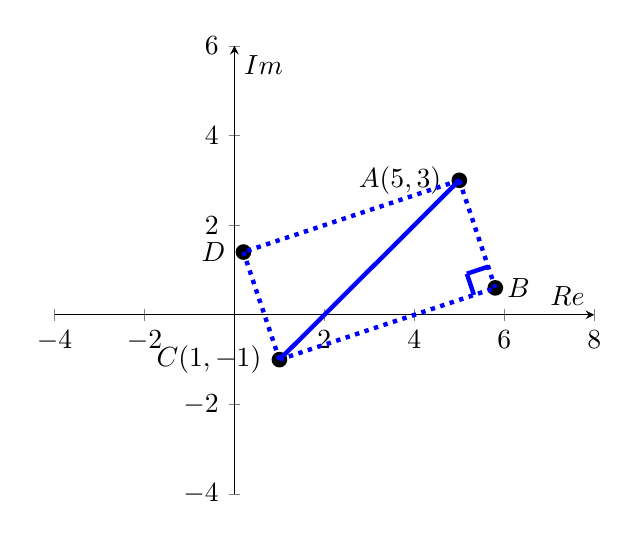
\begin{tikzpicture}
			\begin{axis}[
					axis lines = center,
					xlabel = $Re$,
					ylabel = $Im$,
					xmin = -4, xmax=8, ymin=-4, ymax=6,
				]
				\node[label={180:{$A(5,3)$}},circle,fill,inner sep=2pt] at (axis cs:5,3) {};
				\node[label={180:{$C(1,-1)$}},circle,fill,inner sep=2pt] at (axis cs:1,-1) {};
				\node[circle,fill,inner sep=2pt] at (axis cs:5.8,0.6) {};
				\node[label={180:{$B$}}] at (axis cs:7,0.6) {};
				\node[label={180:{$D$}},circle,fill,inner sep=2pt] at (axis cs:0.2,1.4) {};
				\addplot[mark=none, blue, ultra thick] coordinates {(5,3) (1,-1)}; %AC
				\addplot[mark=none, blue, ultra thick] coordinates {(5.641889117,1.074341649) (5.167544468,0.916227766)};
				\addplot[mark=none, blue, ultra thick] coordinates {(5.325658351,0.441886117) (5.167544468,0.916227766)};
				\addplot[mark=none, blue, ultra thick, dotted] coordinates {(5,3) (5.8,0.6)}; % A to B
				\addplot[mark=none, blue, ultra thick, dotted] coordinates {(5,3) (0.2,1.4)}; %AD
				\addplot[mark=none, blue, ultra thick, dotted] coordinates {(1,-1) (0.2,1.4)}; %CD
				\addplot[mark=none, blue, ultra thick, dotted] coordinates {(1,-1) (5.8,0.6)}; %CB
			\end{axis}
		\end{tikzpicture}

		\begin{align*}
			\textrm{Area of circle }ABCD = \frac{1}{2}\pi r^2
			  & = \frac{1}{2}\pi (\frac{1}{2}|a-c|)^2 \\
			  & = \frac{1}{8}\pi (|5+3i-(1-i)|)^2     \\
			  & = \frac{1}{8}\pi (\sqrt{4^2 + 4^2})^2 \\
			  & = 4\pi \textrm{ units}^2
		\end{align*}
	\end{answer}
	\2 Given that $AB=2BC$ and $AB=CD$, find $b$ and $d$.\hfill[5]
	\begin{answer}
		The vectors $\overrightarrow {BC}$ and $\overrightarrow {BA}$ are represented by complex numbers $c-b$ and $a-b$ respectively. Recall that multiplying a complex number by $i$ gives it a 90-degree anti-clockwise rotation. Given then $BC$ is 2 times of $BA$ and is rotated 90 degrees anti-clockwise from $BA$, we let $b=x+iy$ and we have:
		\begin{align*}
			\overrightarrow {BC} & = (2)(i)\overrightarrow {BA} \\
			c-b                  & = (2i)(a-b)                  \\
			1-i-x-iy             & = 2i(5+3i-x-iy)              \\
			(1-x)+i(-1-y)        & =(2y-6)+i(-2x+10)            \\
		\end{align*}
		Equating real and imaginary parts, $1-x=2y-6$ and $-1-y=10-2x$.\\
		Using a G.C., we obtain $x=5.8,y=0.6$.\\
		$\therefore b=5.8+0.6i$\\
		Since $\overrightarrow {AB} = \overrightarrow {DC}$ we have:
		\begin{align*}
			b-a & = c-d                     \\
			d   & = c-b+a                   \\
			    & = (1-i)-(5.8+0.6i)+(5+3i) \\
			    & = 0.2+1.4i
		\end{align*}
	\end{answer}
\end{outline}

\end{document}
